Для~решения задачи поиска критического пути проекта с нечёткими временными оценками операций, воспользуемся вводимыми в~пп.\,\ref{chapter2_2}, \ref{chapter2_3} преобразованием $L$ и~алгеброй модифицированных нечётких чисел. Для~начала сформулируем задачу для произвольного $\alpha$-уровня. Преобразование $L$, применяемое в~данной задаче, несколько отличается от вводимого в~главе~\ref{chapter2}, поскольку параметры $\lambda$ необходимо изменять, управляя, таким образом, устойчивостью задачи линейного программирования~\cite{Vorontsov_VSTU}:
\begin{equation}
\label{eq:times-l-transform}
  L(\tau_i(\alpha ))=\bar{\tau}_i\left(\alpha, \lambda_{\tau_i}\right)=\lambda_{\tau_i}\tau_{i}^{L}\left(\alpha \right)+(1-\lambda_{\tau_i})\tau_{i}^{R}\left(\alpha \right).
\end{equation}

В формуле \eqref{eq:times-l-transform} границы числа $\tilde \tau_i$ определяются согласно~\eqref{eq:xlxr-to-abm}:
\begin{equation*}
  \left[ \begin{aligned}
    & \tau_{i}^{L}\left(\alpha \right)=m_{\tilde \tau_i}-a_{\tilde \tau_i}+a_{\tilde \tau_i}\alpha; \\ 
    & \tau_{i}^{R}\left(\alpha \right)={{m}_{{{{\tilde{\tau }}}_{i}}}}+{{b}_{{{{\tilde{\tau }}}_{i}}}}-{{b}_{{{{\tilde{\tau }}}_{i}}}}\alpha.
  \end{aligned} \right.
\end{equation*}

В результате, на~каждом из~$\alpha$-уровней задача линейного программирования будет выглядеть следующим образом~\cite{Alushta-2, Vorontsov_VSTU}:
\begin{equation}
\label{eq:modified-fcpm-lp}
  \left\{ \begin{aligned}
    & T(\alpha )=t_n-t_1\to \min  \\ 
    & t_{j_s}-t_{i_s}\geqslant \bar{\tau}_s\left(\alpha,\lambda_s \right),\ \forall s=\overline{1,m}.
  \end{aligned} \right.
\end{equation}

Результатом решения задачи~\eqref{eq:modified-fcpm-lp} является вектор времён $t\left( \alpha \right)=\left\{ t_0\left(\alpha, \lambda_0\right),\ldots,t_n\left(\alpha, \lambda_n\right) \right\}$, который является календарным планом $\alpha$-уровня, а~также множество критических операций $S_1\left( \alpha \right)$~\cite{VSU-2, Alushta-2}.

Нечеткость оценок $\tilde{\tau}_i$ обуславливает проблему устойчивости решений задачи~\eqref{eq:modified-fcpm-lp} в~смысле~\eqref{eq:fuzzy-solution-stability}. Для неустойчивой задачи на различных $\alpha$-уровнях решения соответствуют различным критическим путям, и~возникает проблема объединения разнородных $\alpha$-уровневых решений $S_1\left(\alpha \right)$. Очевидно, что задача будет устойчива, если критический путь не~меняется при переходе с~одного $\alpha$-уровня на~другой. Поэтому целесообразно исследовать задачу~\eqref{eq:modified-fcpm-lp} на~устойчивость и выяснить, при каких значениях параметра $\lambda$ критический путь одинаков на~всех $\alpha$-уровнях~\cite{Vorontsov_VSTU}. Сразу отметим, что при решении задачи~\eqref{eq:modified-fcpm-lp}, будем использовать параметр $\displaystyle \lambda_{s}^{*}=\frac{a_s}{a_s+b_s}$, оптимальный в~смысле сохранения максимального количества характеристик нечёткого числа.

Согласно данному ранее определению~\eqref{eq:fuzzy-solution-stability}, задачу~\eqref{eq:modified-fcpm-lp} поиска критического пути на $\alpha$-уровне будем считать устойчивой по~решению, если она устойчива и если $S_1$ не~зависит от $\alpha$, т.\,е. на всех $\alpha$-уровнях критический путь не изменяется и~проходит по~одним и~тем~же рёбрам. Условие устойчивости выполняется автоматически, поскольку в~сетевом графике всегда существует хотя бы один путь от истока к стоку, следовательно, независимо от величин весов рёбер, всегда существует путь максимальной длины~\cite{Kormen}. Что~касается устойчивости по~решению, то, поскольку результатом решения задачи о~критическом пути является множество номеров критических операций, целесообразно выбрать в~качестве метрики сходства решений мощность симметрической разности двух множеств. Очевидно, что если для $\alpha_1, \alpha_2 \in \left[ 0;1 \right];\ \alpha_1\ne \alpha_2$ $S_1\left( \alpha_1 \right)=S_1\left(\alpha_2 \right)$, то мощность симметрической разности этих множеств $S_1\left( \alpha_1 \right)\Delta S_2\left(\alpha_2 \right)$ равна нулю, т.\,е. критические пути на разных $\alpha$-уровнях совпадают. Подобное условие устойчивости используется и~в~\cite{PhD_Starodubtsev}.

Таким образом, задачу поиска критического пути на $\alpha $-уровне будем считать устойчивой по решению, если она устойчива и если 
\begin{equation}
\label{eq:modified-cpm-lp-stability}
  \forall \alpha_1, \alpha_2\in \left[ 0;1 \right];\ \alpha_1\ne \alpha_2\ S_1\left(\alpha_1 \right)\Delta S_2\left(\alpha_2 \right)=\varnothing,
\end{equation}
т.\,е. на всех $\alpha $-уровнях критический путь не~изменяется и~проходит по~одним и~тем~же дугам. 

В~п.\,\ref{chapter2_3} было показано, что ввиду линейности преобразования $L$, для получения функции принадлежности модифицированного нечёткого числа, достаточно знать его значения в~двух точках~--- при~$\alpha=0$ и~$\alpha=1$. На~этом основывается упрощённый способ решения задачи. В~качестве невозмущённой задачи возьмём исходную задачу~\eqref{eq:modified-fcpm-lp} при $\alpha=1$. Возмущения возникают при изменении $\alpha$ и~$\lambda$, поскольку в~этом случае меняется чёткое значение числа на~каждом $\alpha$-срезе. На устойчивость задачи можно влиять, изменяя параметры $\lambda$ для каждого из чисел. Для дальнейшего анализа задачи~\eqref{eq:modified-fcpm-lp} на~устойчивость достаточно решить её при~$\alpha=1$, а~затем, зафиксировав полученный критический путь с~помощью изменения части ограничений на~строгие равенства для~соответствующих~операций, проверить существование решения при $\alpha=0$ и~степень его~совпадения с~решением при $\alpha=1$.

Полученное при $\alpha=1$ решение задачи~\eqref{eq:modified-fcpm-lp} даёт активные ограничения на критические операции. Кроме того, в~п.~\ref{chapter2_4} было отмечено, что на параметры $\lambda_S$ преобразования $L$ также необходимо наложить ограничения и учесть их в целевой функции~\eqref{eq:modified-target-function}, чтобы избежать ситуации, когда $\lambda_S$ принимают граничные значения (0 или 1)~\cite{Vorontsov_VSTU}. В~результате при $\alpha=0$ решается видоизменённая задача
\begin{equation}
\label{eq:modified-fcpm-lp-alpha}
  \left \{ \begin{aligned}
    & T^* \left(\alpha, \lambda \right) = t_n-t_1+\gamma \sum \limits_{s=1}^{m} \left(\lambda_s^*-\lambda_s \right)^2 \to \min; \\
    & t_{j_{s_1}}-t_{i_{s_1}} = \bar{\tau}_{s_1}\left(\alpha, \lambda_{s_1} \right),\ \forall s_1 \in S_1\left(1\right); \\
    & t_{j_s}-t_{i_s} \geqslant \bar{\tau}_s\left(\alpha, \lambda_s \right),\ \forall s \notin S_1\left(1\right),\,s=\overline{1,m}.
  \end{aligned} \right.
\end{equation}

В~итоге, для решения задачи поиска критического пути~\eqref{eq:modified-fcpm-lp} предлагается использовать следующий алгоритм~\cite{Vorontsov_VSTU}.
\begin{enumerate}
  \item Решается невозмущённая задача~\eqref{eq:modified-fcpm-lp} при~$\alpha=1$. Ввиду свойства~\ref{prop:L-prop1} преобразования $L$, это решение соответствует модифицированному решению $\left \langle T\left(1\right), t\left(1\right), S_1\left(1\right) \right \rangle$. Фиксируется множество операций $S_1\left(1\right)$, образующих критический путь.
  \item Фиксируется критический путь при всех $\alpha \neq 1$. Для этого в~задаче~\eqref{eq:modified-fcpm-lp} нестрогие неравенства меняются на равенства $\forall s_1 \in S_1\left(1\right)$, т.\,е. выбранные операции всегда будут иметь нулевой резерв времени~\eqref{eq:full-work-reserve}. Данный шаг позволяет выполнить условие устойчивости задачи по решению~\eqref{eq:modified-cpm-lp-stability}.
  \item Решается возмущённая задача~\eqref{eq:modified-fcpm-lp-alpha} c~изменённой целевой функцией. Результатом решения задачи является кортеж $\left \langle T\left(0\right), t\left(0\right), \lambda \right \rangle$, где $\lambda$~--- вектор параметров преобразования $L$.
  \item Решение исходной задачи представляет из себя тройку $\left \langle \tilde T, S_1, \lambda \right \rangle$. Функция принадлежности общего времени выполнения проекта $\tilde T$ восстанавливается по значениям $T\left(0\right)$ и $T\left(1\right)$, либо число $\tilde T$ оставляется в~виде~\eqref{eq:modified-number-base}.
\end{enumerate}
  
Рассмотрим алгоритм решения на примере и сравним его результаты с результатами некоторых других методов, описанных в~п.\,\ref{chapter3_1}.

\textbf{Пример.} Пусть дан проект, заданный таблицей~\ref{t:sample-project-estimates}. Требуется определить критические операции проекта, а~также его общее нечёткое время выполнения.

\begin{table}[b!]
\caption{Оценки длительностей операций проекта и их взаимосвязи}
\label{t:sample-project-estimates}
\begin{center}
\begin{tabularx}{0.8\textwidth}{|p{0.15\linewidth}|X|p{0.1\linewidth}|p{0.1\linewidth}|p{0.1\linewidth}|}
	\hline
		\centering \textit{Операция} & \centering \textit{Предшествующие операции} & \centering \textit{a} & \centering \textit{m} & \centering \textit{b} \tabularnewline	\hline
	\hline
		A & -   & 1 & 2  & 3 \tabularnewline \hline
		B & -   & 2 & 4  & 1 \tabularnewline \hline
		C & A   & 4 & 7  & 2 \tabularnewline \hline
		D & B   & 2 & 6  & 3 \tabularnewline \hline
		E & B   & 1 & 10 & 2 \tabularnewline \hline
		F & C   & 1 & 5  & 1 \tabularnewline \hline
		G & D,E & 4 & 5  & 1 \tabularnewline \hline
		H & F,G & 2 & 4  & 3 \tabularnewline
    \hline
\end{tabularx}
\end{center}
\end{table}

Вначале выпишем $L$-преобразование для каждой нечёткой временной оценки:
\begin{equation}
\label{eq:sample-project-L-transform}
\left[ \begin{aligned}
   & \bar{\tau}_A\left( \alpha \right)=\lambda_A\left( 1+\alpha \right)+\left( 1-\lambda_A \right)\left( 5-3\alpha \right) \\ 
   & \bar{\tau}_B\left( \alpha \right)=\lambda_B\left( 2+2\alpha \right)+\left( 1-\lambda_B \right)\left( 5-\alpha \right) \\ 
   & \bar{\tau}_C\left( \alpha \right)=\lambda_C\left( 3+4\alpha \right)+\left( 1-\lambda_C \right)\left( 9-2\alpha \right) \\ 
   & \bar{\tau}_D\left( \alpha \right)=\lambda_D\left( 4+2\alpha \right)+\left( 1-\lambda_D \right)\left( 9-3\alpha \right) \\ 
   & \bar{\tau}_E\left( \alpha \right)=\lambda_E\left( 9+\alpha \right)+\left( 1-\lambda_E \right)\left( 12-2\alpha \right) \\ 
   & \bar{\tau}_F\left( \alpha \right)=\lambda_F\left( 4+\alpha \right)+\left( 1-\lambda_F \right)\left( 6-\alpha \right) \\ 
   & \bar{\tau}_G\left( \alpha \right)=\lambda_G\left( 1+4\alpha \right)+\left( 1-\lambda_G \right)\left( 6-\alpha \right) \\ 
   & \bar{\tau}_H\left( \alpha \right)=\lambda_H\left( 2+2\alpha \right)+\left( 1-\lambda_H \right)\left( 7-3\alpha \right)
\end{aligned} \right.
\end{equation}

Соответствующий сетевой график изображён на рисунке~\ref{fig:pplan}. Из~него видно, что для~корректного отображения зависимостей между операциями, введена фиктивная операция Ф1 длительностью 0 дней.
\begin{figure}[h!]
  \centering
  {
    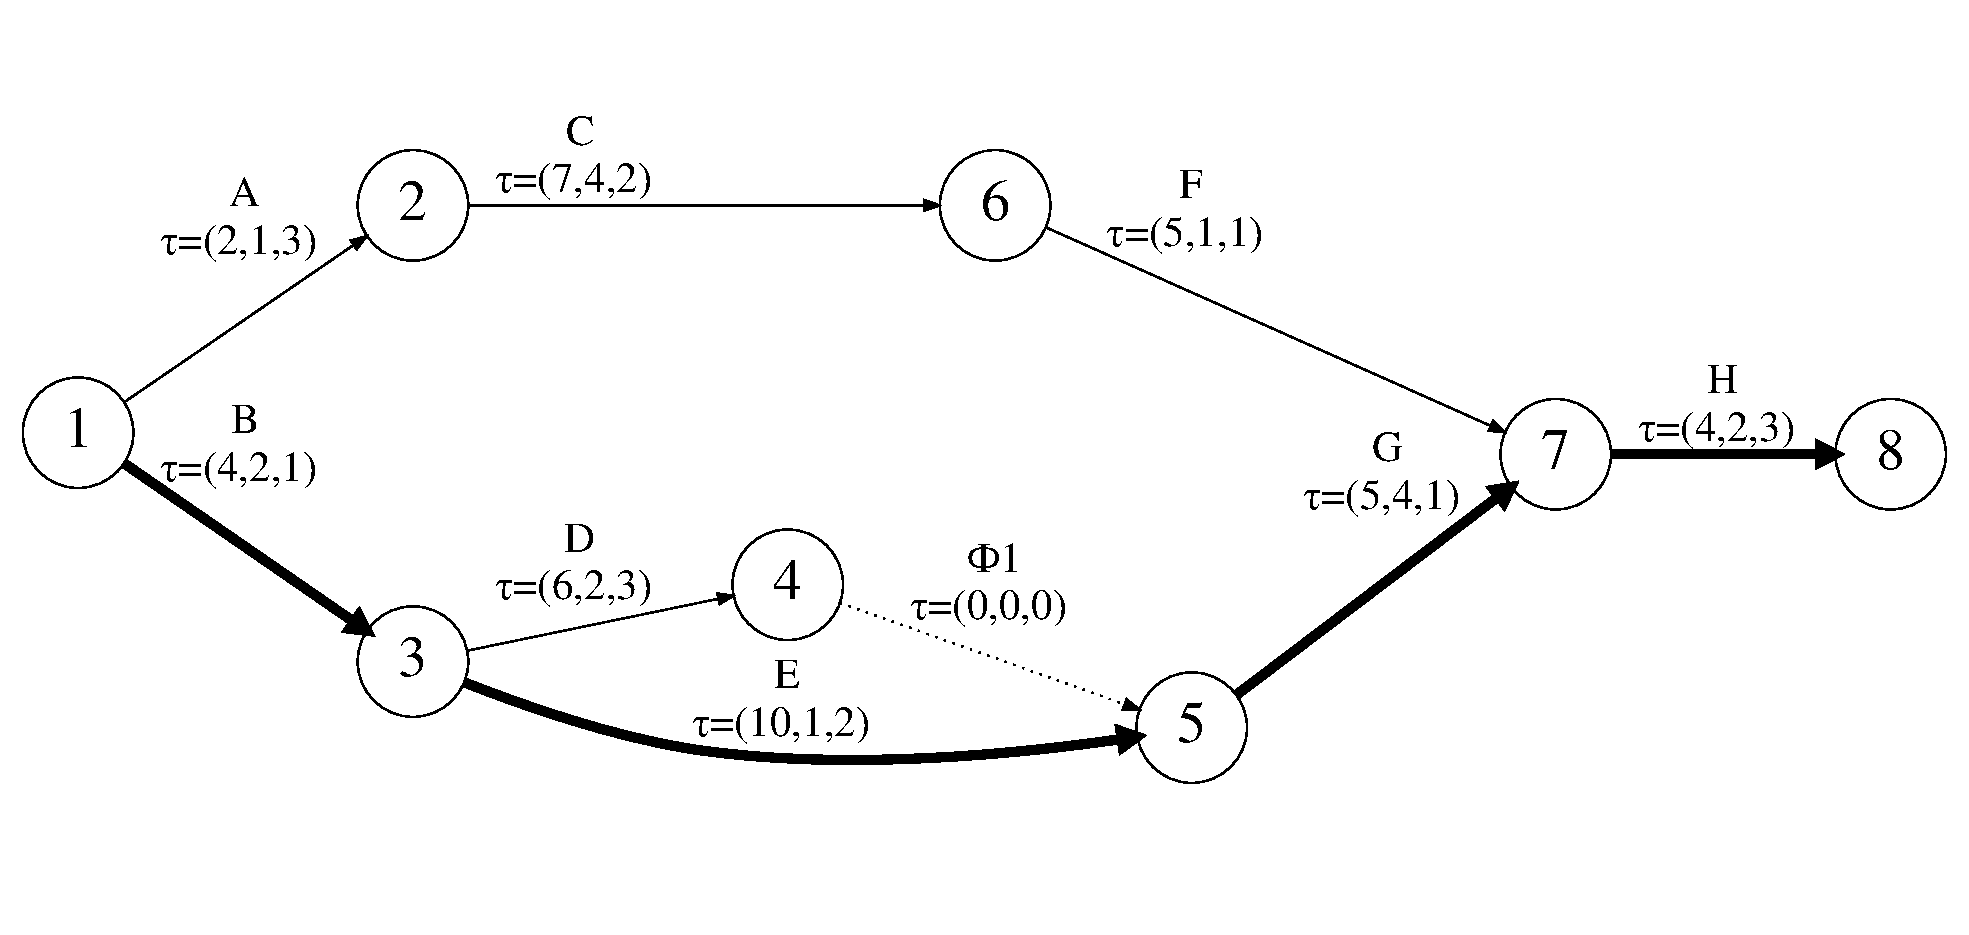
\includegraphics[width=0.9\textwidth]{pplan}
    \caption{Cетевой график проекта с нечёткими временными оценками}
    \label{fig:pplan}
  }
\end{figure}

Для решения задачи можно воспользоваться любым математическим пакетом или встраиваемым модулем, поддерживающим решение задач линейного программирования (в рассматриваемом примере использовалась надстройка <<Поиск решения>> в Microsoft Excel). Решая задачу~\eqref{eq:modified-fcpm-lp} с~учётом~\eqref{eq:sample-project-L-transform} при~$\alpha=1$, получаем:
\begin{gather*}
  T\left( 1 \right)=23; \\ 
  t\left( 1 \right)=\left\{ 0;7;4;14;14;14;19;23 \right\}; \\ 
  S_1\left( 1 \right)=\left\{ B,E,G,H \right\}.
\end{gather*}

После этого решаем задачу~\eqref{eq:modified-fcpm-lp-alpha}, которая с~учётом~\eqref{eq:sample-project-L-transform} при~$\alpha=0$ принимает вид
\begin{equation}
\label{eq:0-level-fcpm-task}
  T\left( 0 \right)=t_8-t_1+\gamma \sum\limits_{s=1}^{8}\left( \lambda_{s}^{*}-\lambda_s \right)^{2}\to \min
\end{equation}
\begin{equation}
\label{eq:0-level-fcpm-constraints}
  \left\{ \begin{aligned}
    & t_2-t_1 \geqslant 5-4\lambda_A \\ 
    & t_3-t_1=5-3\lambda_B \\ 
    & t_6-t_2 \geqslant 9-6\lambda_C \\ 
    & t_4-t_3 \geqslant 9-5\lambda_D \\ 
    & t_5-t_3=12-3\lambda_E \\ 
    & t_5-t_4 \geqslant 0 \\ 
    & t_7-t_6 \geqslant 6-2\lambda_F \\ 
    & t_7-t_5=6-5\lambda_G \\ 
    & t_8-t_7=7-5\lambda_H
  \end{aligned} \right.
\end{equation}

Значение $\gamma$ выбирается порядка 10. В~результате решения задачи~\eqref{eq:0-level-fcpm-task} при~ограничениях~\eqref{eq:0-level-fcpm-constraints} получаем, что
\begin{gather*}
  T^*\left( 0 \right)=20,83; \\
  t\left(0\right)=\left\{ 0;\ 4,23;\ 2,96;\ 13,92;\ 13,92;\ 9,97;\ 15,79;\ 20,67 \right\}; \\ 
  S_1\left( 0 \right)=\left\{ B,E,G,H \right\}; \\ 
  \lambda =\left\{ 0,25;\ 0,68;\ 0,67;\ 0,4;\ 0,35;\ 0,5;\ 0,83;\ 0;43 \right\}.
\end{gather*}

В~итоге имеем критический путь $S_1=\left\{ B,E,G,H \right\}$ и~нечёткое время выполнения $T\left( \alpha \right)=20,67+2,33\alpha$.

При решении задачи согласно способам второй группы, описываемым в~\cite{Chinese_CPM, FCPA_Ravi_Shankar, Indians_FCPM}, используется функция ранжирования Ягера~\eqref{eq:yager-ranking-lp-helper}, которая для треугольных чисел равна
\begin{equation}
  I\left( \tilde A \right) = \frac{1}{2} \int \limits_{0}^{1} \left(m-a+a\alpha+m+b-b\alpha \right) d\alpha = m+\frac{b-a}{4}.
\end{equation}

Для проекта, описываемого таблицей~\ref{t:sample-project-estimates}, задача целочисленного программирования~\eqref{eq:yager-ranking-lp-cpm}--\eqref{eq:lp-cpm-int-constraints} выглядит следующим образом:
\begin{gather*}
  I\left( \tilde T \right) = 2,5x_{12}+3,75x_{13}+6,5x_{26}+6,25x_{34}+10,25x_{35}+{}\\
  {}+4,25x_{57}+5x_{67}+4,25x_{78} \to max;
\end{gather*}
\begin{equation*}
  \left \{ \begin{aligned}
    & x_{12} + x_{13} = 1; \\
    & x_{12} = x_{26}; \\
    & x_{13} = x_{34} + x_{35}; \\
    & x_{34} = x_{45}; \\
    & x_{35} + x_{45} = x_{57}; \\
    & x_{26} = x_{67}; \\
    & x_{67} + x_{57} = x_{78}; \\
    & x_{78} = 1.
  \end{aligned} \right.
\end{equation*}

Решение задачи даёт следующие значения, в~целом соответствующие модифицированному решению:
\begin{gather*}
  x_{12}=x_{26}=x_{34}=x_{45}=x_{67}=0; \\
  x_{13}=x_{35}=x_{57}=x_{78}=1; \\
  S_1=\left \{ B,E,G,H \right\}; \\
  \tilde T = \tilde \tau_B + \tilde \tau_E + \tilde \tau_G + \tilde \tau_H = \left \langle 23; 9; 7 \right \rangle.
\end{gather*}

Решение с помощью метода~\cite{Uskov_FCPM, Dubois_Prade} позволяет найти только общее время выполнения проекта. Выполняя прямой проход по~графу и~используя формулы~\eqref{eq:fcpm-dubois-max}, получим:
\begin{gather*}
  t_1^{-} = 0; \\
  t_2^{-} = t_1^{-}+\tau_A = \left \langle 2;1;3 \right \rangle; \\
  t_3^{-} = t_1^{-}+\tau_B = \left \langle 4;2;1 \right \rangle; \\
  t_4^{-} = t_3^{-}+\tau_D = \left \langle 10;4;4 \right \rangle; \\
  t_5^{-} = \max \left \{ t_3^{-}+\tau_E; t_4^{-} \right \} = \max \left\{ \left \langle 14;3;3 \right \rangle; \left \langle 10;4;4 \right \rangle \right\} = \left \langle 14;3;3 \right \rangle; \\
  t_6^{-} = t_2^{-}+\tau_C = \left \langle 9;5;5 \right \rangle; \\
  t_7^{-} = \max \left \{ t_5^{-}+\tau_G; t_6^{-}+\tau_F \right \} = \max \left\{ \left \langle 19;7;4 \right \rangle; \left \langle 14;6;6; \right \rangle \right\} = \left \langle 19;7;4 \right \rangle; \\
  T = t_8^{-} = t_7^{-} + \tau_H = \left \langle 23;9;7 \right \rangle.
\end{gather*}
Обратный проход по графу приведёт к~тому, что нечёткость времён выполнения будет учтена дважды, поэтому можно воспользоваться формулой для наиболее поздних сроков наступления событий из~\cite{Leondes}:
\begin{equation}
\label{eq:leondes-let-fcpm}
  t_i^{+} = \underset{l}{\max} \left\{ t_i^{-}; \underset{s}{\min} \left(r_l - q_s\left(i \right) \right) \right \},
\end{equation}
где $r_l$~--- вес пути, проходящего через вершину $i$, от~истока к~стоку, а~$q_s$~--- вес пути от~текущего события до стока. Для~стока принимается, что~$t_n^{+}=t_n^{-}$. При~этом ведутся достаточно трудоёмкие вычисления с получением таблиц возможных наиболее поздних сроков для каждого события и~используется способ выбора максимального из~двух чисел~\eqref{eq:mccaloh-lee-comparison}, описанный в~\cite{McCahon_Lee}.

В~графе, описываемом таблицей~\ref{t:fuzzy-modeling-approaches}, существуют три возможных пути от~истока к~стоку~--- 1-2-6-7-8, 1-3-4-5-7-8, 1-3-5-7-8. Их~длины равны
\begin{gather*}
  r_1 = \tau_A+\tau_C+\tau_F+\tau_H = \left \langle 18; 8; 9 \right \rangle; \\
  r_2 = \tau_B+\tau_D+\tau_{\Phi 1}+\tau_G+\tau_H = \left \langle 19; 10; 8 \right \rangle; \\
  r_3 = \tau_B+\tau_E+\tau_G+\tau_H = \left \langle 23; 9; 7 \right \rangle.
\end{gather*}
Для вершины 7 расстояние $q_s\left(i\right) = \tau_H = \left \langle 4;2;3  \right \rangle$, минимальная разность $r_l - q_s\left(i \right)$ равна $\left \langle 15; 13; 10 \right \rangle$, поэтому, согласно формулам~\eqref{eq:leondes-let-fcpm} и~\eqref{eq:mccaloh-lee-comparison}
\begin{equation*}
  t_7^{+}=\max \left\{ \left \langle 19;7;4 \right \rangle; \left \langle 15;13;10 \right \rangle \right\} = \left \langle 19;7;4 \right \rangle.
\end{equation*}

Для остальных событий расчёт аналогичен. В конечном итоге получается, что критическим со степенью, равной единице, является путь $\left\{B, E, G, H \right\}$. Данный пример подтверждает соответствие модифицированного решения полному, полученному с~использованием методов второй группы из~\cite{Leondes, Dubois_Prade, McCahon_Lee}.